\documentclass{beamer}

\mode<presentation>{\usetheme{Madrid}}
\usepackage{graphicx}
\usepackage{multimedia}
\usepackage{hyperref}

\usepackage[utf8]{inputenc}
\usepackage[ngerman]{babel}
\usepackage{amsmath, amssymb, amsthm}

\usepackage{subcaption}
\usepackage[T1]{fontenc}
%\usepackage[sort&compress]{natbib}

\usepackage{lmodern}
\usepackage{caption}


\author[Philipp Geier]{}
\title[]{2. Übung zur Vorlesung
Software Architectures for Enterprises\\
Santa Claus needs your help!}
\institute[Universität Trier]{}
\date[28. Januar 2024]{}
\beamertemplatenavigationsymbolsempty
\setbeamertemplate{footline}
{
  \leavevmode%
  \hbox{%
  \begin{beamercolorbox}[wd=.50\paperwidth,ht=2.25ex,dp=1ex,center]{author in head/foot}%
    \usebeamerfont{author in head/foot}\insertshortauthor%~~\beamer@ifempty{\insertshortinstitute}{}{(\insertshortinstitute)}
  \end{beamercolorbox}%
  \begin{beamercolorbox}[wd=.50\paperwidth,ht=2.25ex,dp=1ex,right]{date in head/foot}%
    \usebeamerfont{date in head/foot}\insertshortdate{}\hspace*{2em}
    \insertframenumber{} / \inserttotalframenumber\hspace*{2ex} 
  \end{beamercolorbox}}%
  \vskip0pt%
}
%—-------------------------------------------------------------

\begin{document}
{
  \usebackgroundtemplate{ 
\includegraphics[width=\paperwidth]{Santa}}
  \begin{frame}
    \maketitle
  \end{frame}
}
    
    %\begin{frame}
       % \frametitle{Inhalt}
		%\tableofcontents
	%\end{frame}
	
%—------------------------------------------------------

\begin{frame}{XmasWishes \cite{a}}
\begin{figure}
\vspace*{-.8cm}
\hspace*{-1cm}

\includegraphics[width=1.1\paperwidth]{Designer}
\caption{Gameplay}
\end{figure}
\end{frame}

\begin{frame}{Modellierung}
\begin{figure}
    \centering
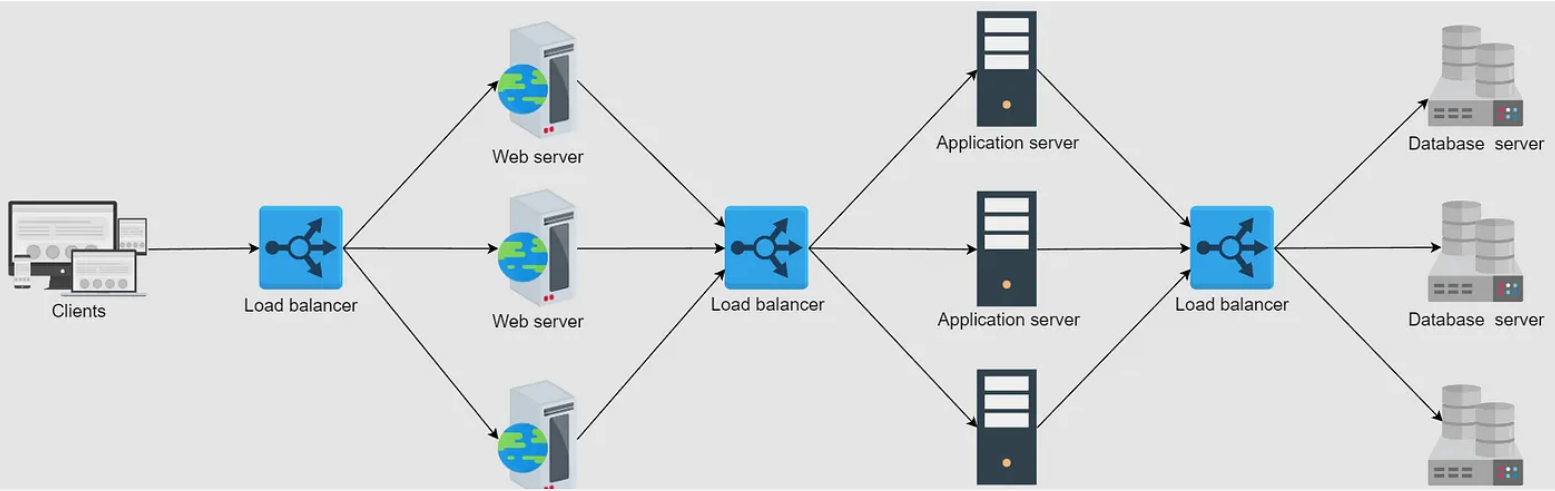
\includegraphics[width=\textwidth, keepaspectratio]{loads}
\caption{Modellierung \cite{b}}
\end{figure}
\end{frame}

\begin{frame}{Konkretisierung}
\begin{figure}
    \centering
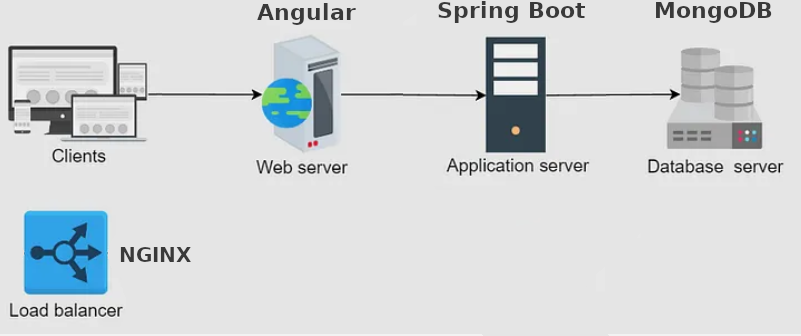
\includegraphics[width=\textwidth, keepaspectratio]{proto}
\caption{Konkretisierung \cite{b}}
\end{figure}
\end{frame}

\begin{frame}{Prototyp}
\begin{figure}
    \centering
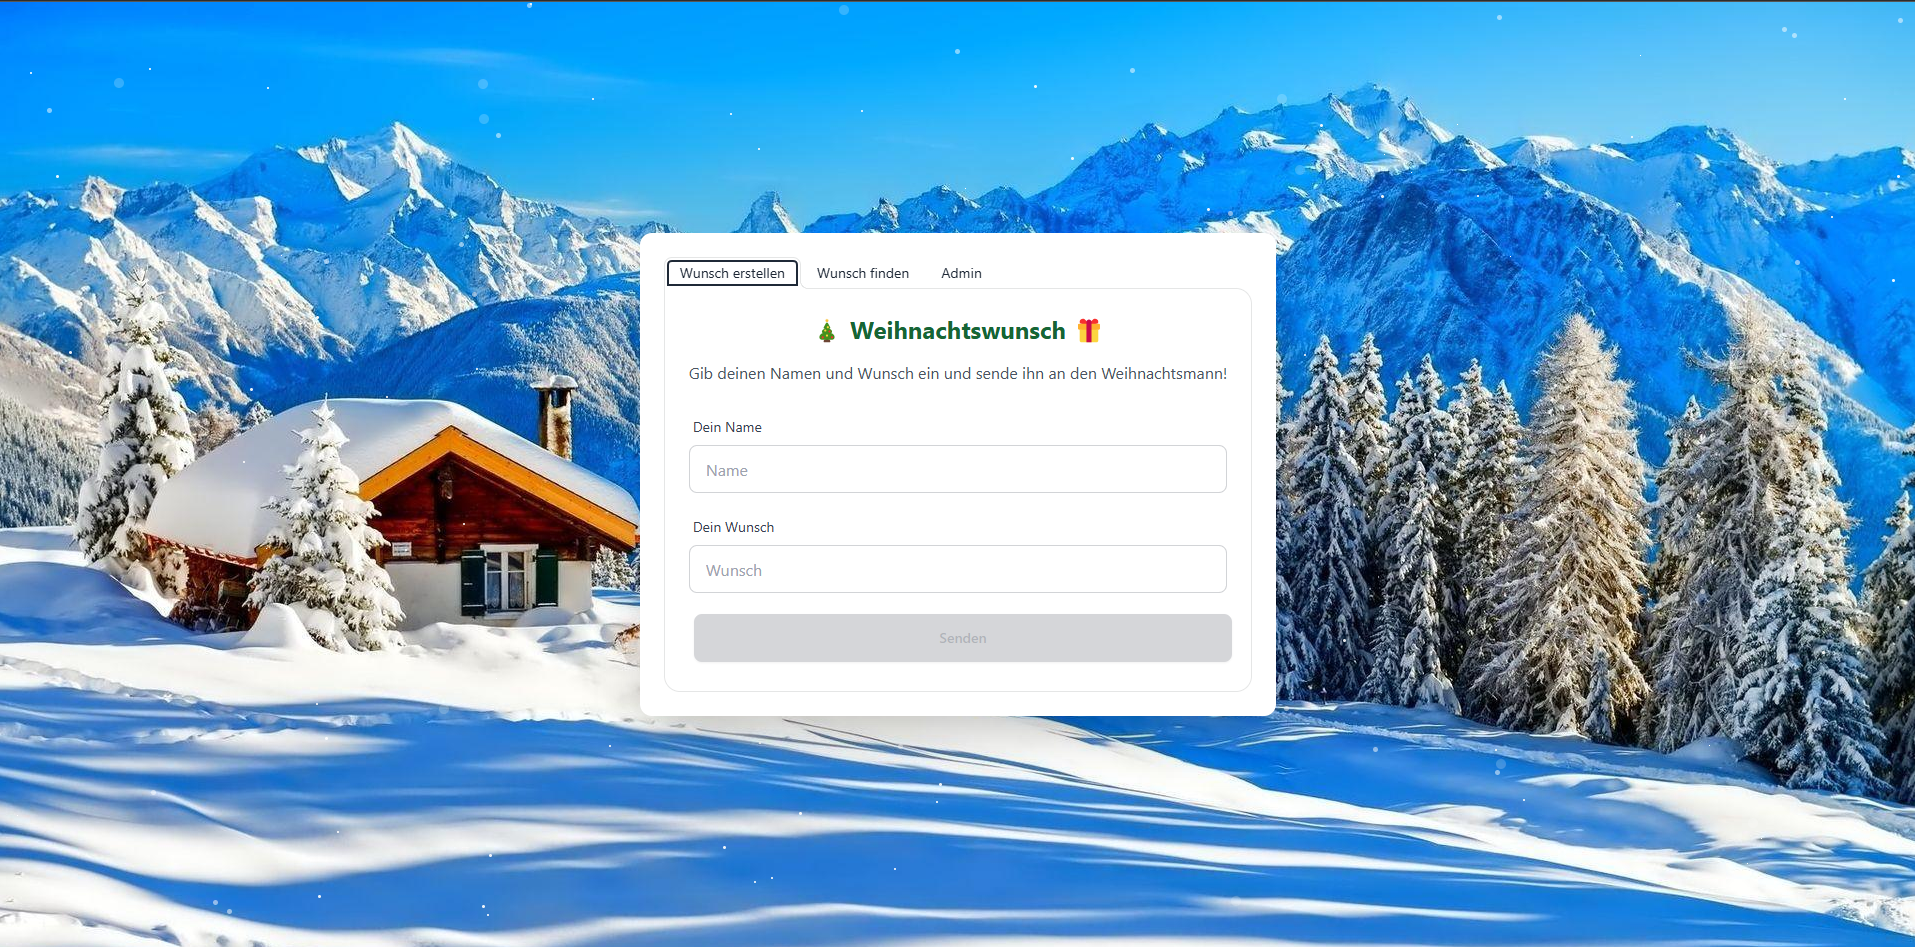
\includegraphics[width=\textwidth, keepaspectratio]{funk1}
\caption{Wunsch erstellen \cite{f}\cite{g}}
\end{figure}
\end{frame}

\begin{frame}{Prototyp}
\begin{figure}
    \centering
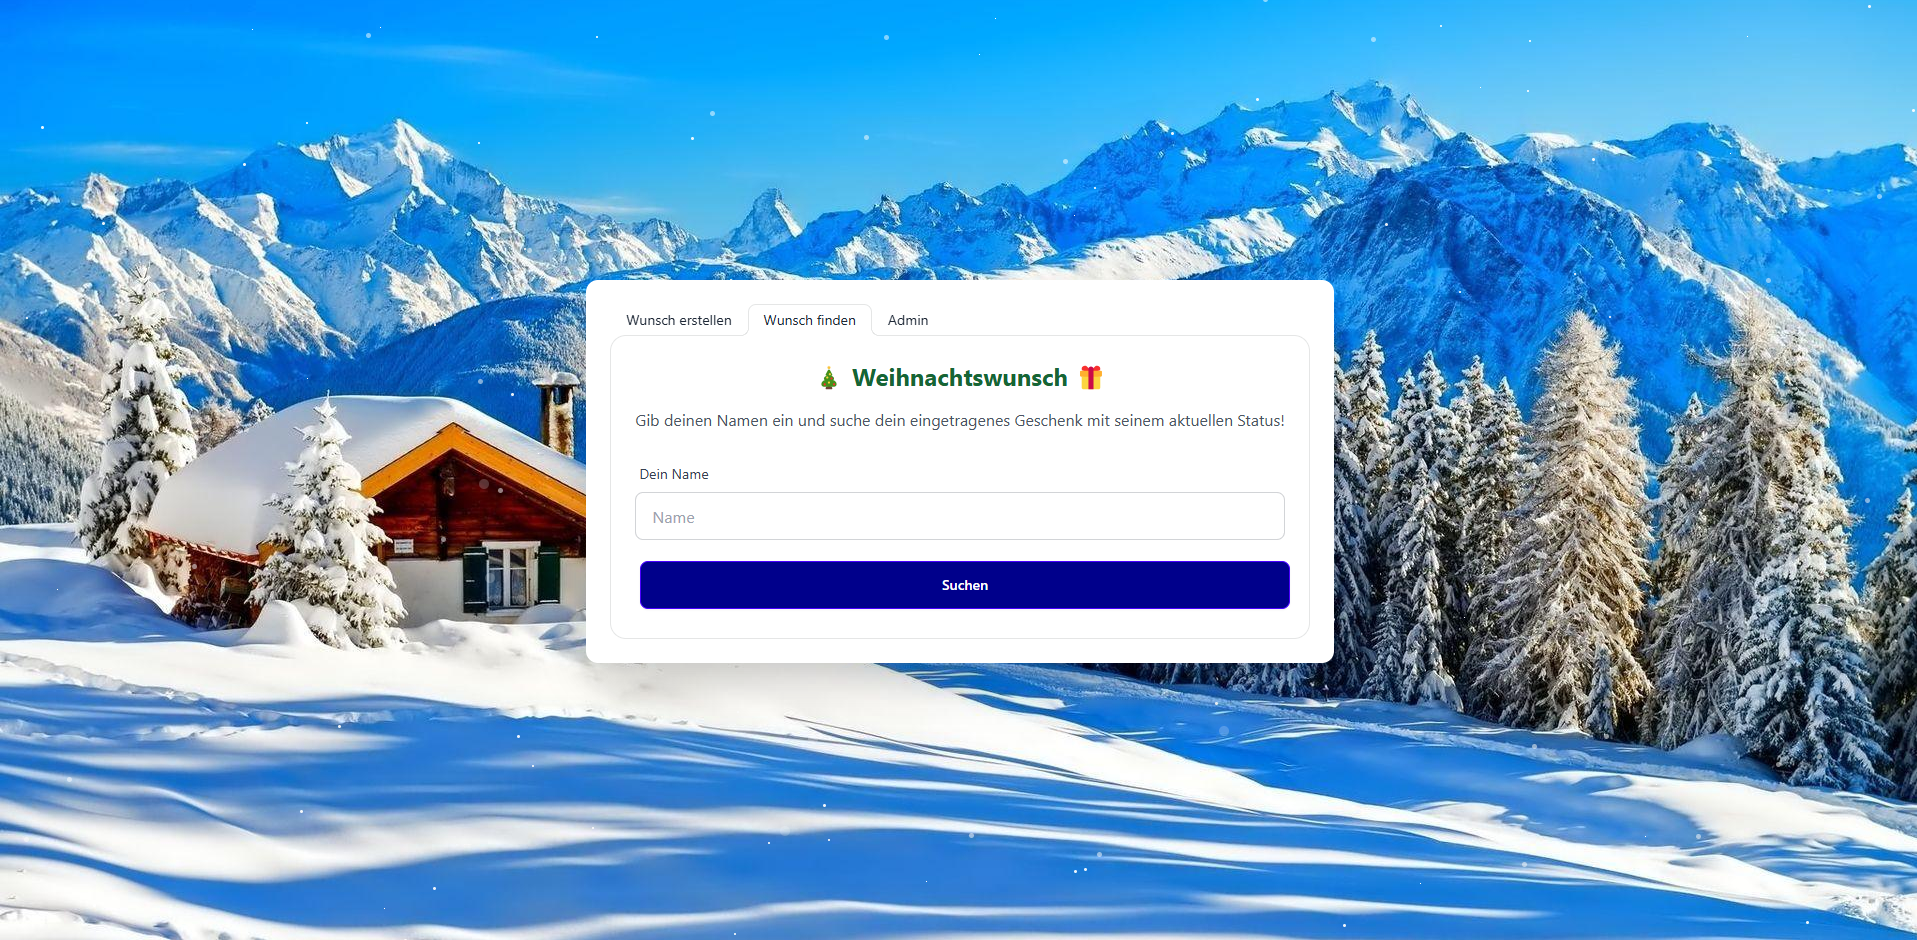
\includegraphics[width=\textwidth, keepaspectratio]{funk2}
\caption{Wunsch finden \cite{f}\cite{g}}
\end{figure}
\end{frame}

\begin{frame}{Prototyp}
\begin{figure}
    \centering
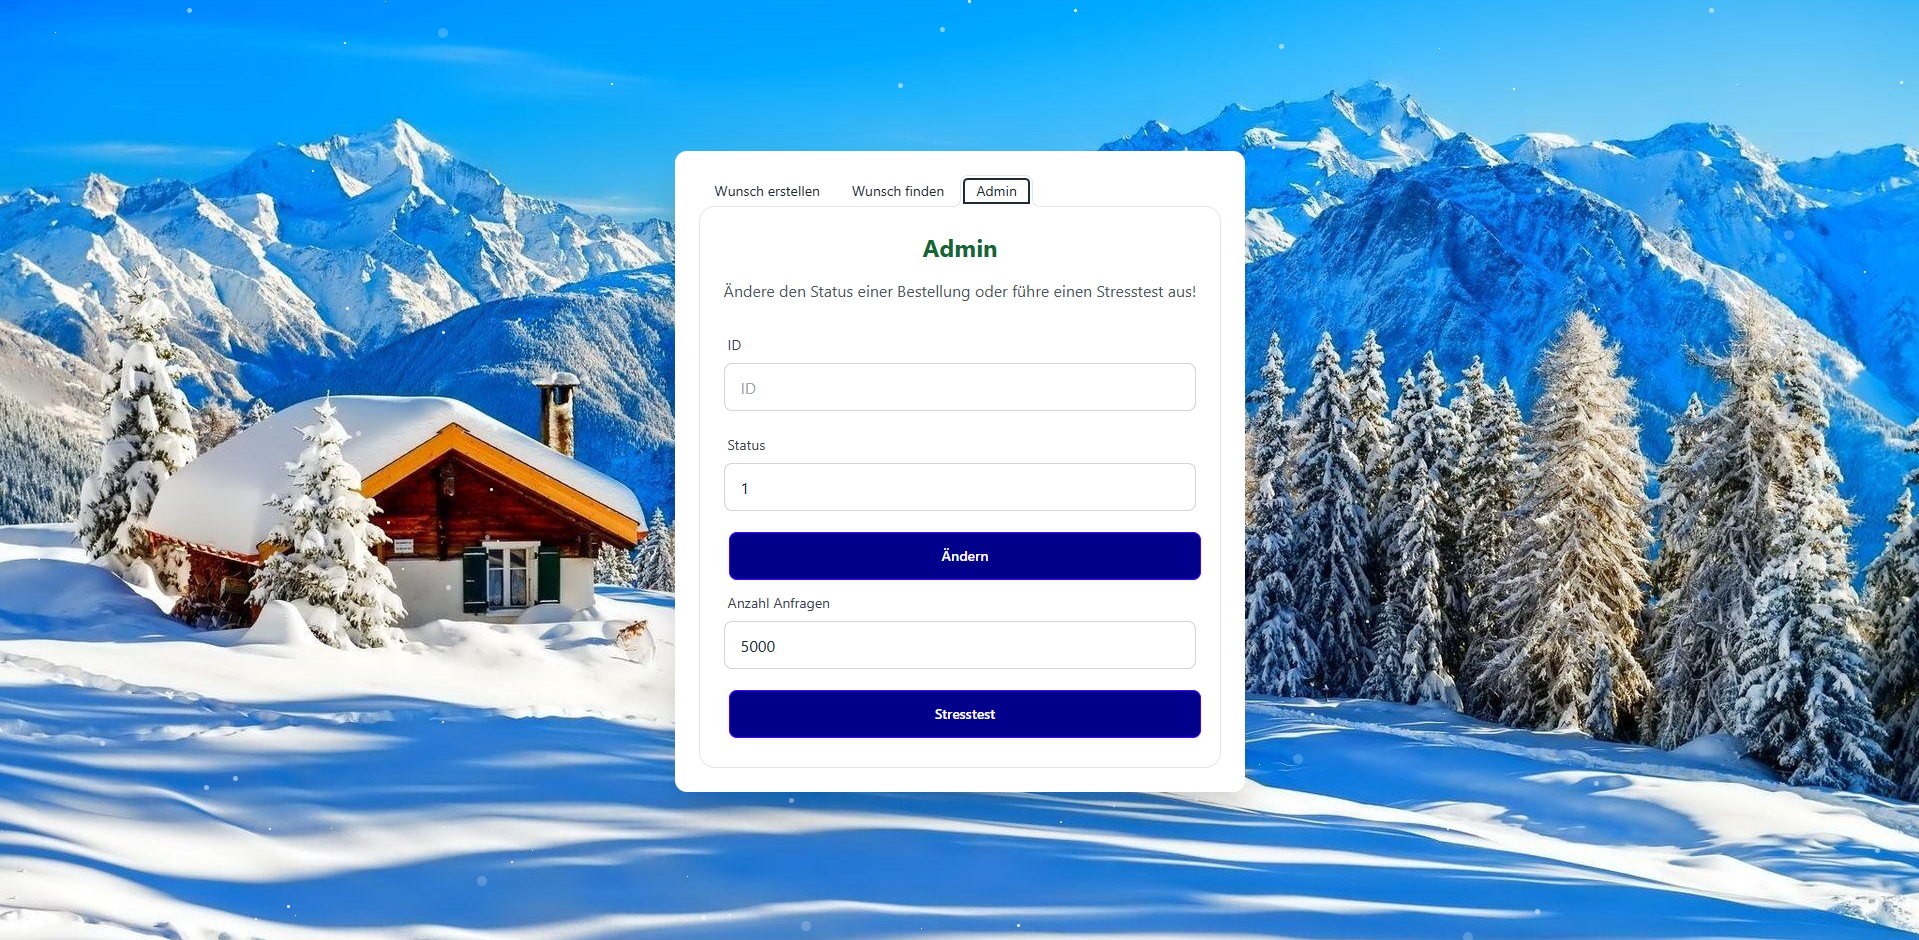
\includegraphics[width=\textwidth, keepaspectratio]{funk3}
\caption{Admin \cite{f}\cite{g}}
\end{figure}
\end{frame}

\begin{frame}{Apache Camel}
\begin{figure}
    \centering
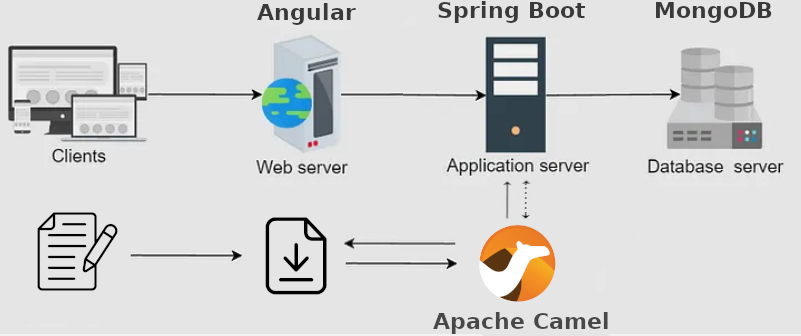
\includegraphics[width=\textwidth, keepaspectratio]{apachecamel}
\caption{Apache Camel \cite{c}\cite{d}\cite{e}}
\end{figure}
\end{frame}

\begin{frame}{Quellen}
	\begin{thebibliography}{1}
\bibitem{a}[1]{ \url{https://designer.microsoft.com/image-creator}}
\bibitem{b}[2]{ \url{https://medium.com/@alexeynovikov_89393/load-balancer-theoretical-minimum-4cec4590f237}}
\bibitem{f}[3]{ \url{https://github.com/bennadel/JavaScript-Demos/tree/master/demos/snow-fall-angular11}}
\bibitem{g}[4]{ \url{https://wallpaperaccess.com/winter-mountain}}
\bibitem{c}[5]{ \url{https://encrypted-tbn0.gstatic.com/images?q=tbn:ANd9GcQcl4nb7bx7Jif1Nsup0Fdae7kzKFiXSto2uQ&s}}
\bibitem{d}[6]{ \url{https://cdn-icons-png.flaticon.com/512/7659/7659588.png}}
\bibitem{e}[7]{ \url{https://cdn-icons-png.flaticon.com/512/1092/1092004.png}}

\end{thebibliography}
\end{frame}


	
    	
    	
    	
\end{document}
